%! TeX program = lualatex
\documentclass[a4paper]{article} 

% packages
\usepackage{microtype}      % Slightly tweak font spacing for aesthetics
\usepackage[english]{babel} % Language hyphenation and typographical rules
\usepackage[final, colorlinks = false, urlcolor = cyan]{hyperref} 
\usepackage{changepage}     % adjust margins on the fly
\usepackage{fontspec}

\usepackage{minted}
\usemintedstyle{algol_nu}
\usepackage{xcolor}

\usepackage{pgfplots}
\pgfplotsset{width=\textwidth,compat=1.9}

\usepackage{caption}
\newenvironment{code}{\captionsetup{type=listing}}{}
\captionsetup[listing]{skip=0pt}
\setlength{\abovecaptionskip}{5pt}
\setlength{\belowcaptionskip}{5pt}

\usepackage[yyyymmdd]{datetime}
\renewcommand{\dateseparator}{--}
\setmainfont{EB Garamond}
\setmonofont[Scale=MatchLowercase]{Deja Vu Sans Mono}

\usepackage{titlesec}
% \titleformat{\section}{\LARGE\bfseries}{}{}{}[\titlerule]
% \titleformat{\subsection}{\Large\bfseries}{}{0em}{}
% \titlespacing{\subsection}{0em}{-0.7em}{0em}
%
% \titleformat{\subsubsection}{\large\bfseries}{}{0em}{$\bullet$ }
% \titlespacing{\subsubsection}{1em}{-0.7em}{0em}

% margins
\addtolength{\hoffset}{-2.25cm}
\addtolength{\textwidth}{4.5cm}
\addtolength{\voffset}{-3.25cm}
\addtolength{\textheight}{5cm}
\setlength{\parskip}{0pt}
\setlength{\parindent}{0in}
% \setcounter{secnumdepth}{0}

\begin{document}
\hrule \medskip
\begin{minipage}{0.295\textwidth} 
    \raggedright
    \footnotesize 
    Name: Andrew Hayes \\
    E-mail: \href{mailto://a.hayes18@universityofgalway.ie}{\texttt{a.hayes18@universityofgalway.ie}}  \hfill\\   
    ID: 21321503 \hfill
\end{minipage}
\begin{minipage}{0.4\textwidth} 
    \centering 
    \vspace{0.4em}
    \Large 
    \textbf{CT331} \\ 
\end{minipage}
\begin{minipage}{0.295\textwidth} 
    \raggedleft
    \today
\end{minipage}
\medskip\hrule 
\begin{center}
    \normalsize
    Assignment 2: Functional Programming with Scheme
\end{center}
\hrule

\section{Question 1}
\subsection{Part (A): Code}
\begin{code}
\inputminted[texcl, mathescape, breaklines, frame=single]{racket}{../code/assignment_q1.rkt}
\caption{\texttt{assignment\_q1.rkt}}
\end{code}

\subsection{Part (B): Comments}
\begin{figure}[H]
    \centering
    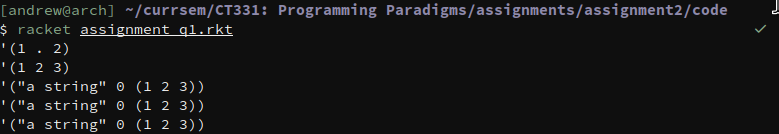
\includegraphics[width=\textwidth]{./images/question1.png}
    \caption{Output of \texttt{assignment\_q1.rkt}}
\end{figure}

Comments on each line of output:
\begin{enumerate}
    \item   The \mintinline{racket}{cons} function creates a \mintinline{racket}{cons} pair, which is not always a ``list''. 
            A list is a \mintinline{racket}{cons} pair in which the second element is another itself another list or is \mintinline{racket}{empty}.
            When a \mintinline{racket}{cons} pair that is not a list is printed, its elements are delimited by a ``\verb|.|'', as can be seen from the first line of
            output.

    \item   The second section of code produces a list of three numbers using only the \mintinline{racket}{cons} function: 
            first we create a one-element list with \mintinline{racket}{(cons 3 empty)}, then we create a two-element list by making a \mintinline{racket}{cons} pair
            of \mintinline{racket}{2} and the already-created one-element list, and finally we create a three-element list by making a \mintinline{racket}{cons} pair
            of \mintinline{racket}{1} and the two-element list.
            This could of course be achieved far more simply by just using \mintinline{racket}{(cons 1 '(2 3))} or even justs \mintinline{racket}{'(1 2 3)} but I
            felt that this would be against the spirit of the exercise.
    
    \item   To create a nested list using only \mintinline{racket}{cons} in the third section of code, we make the \mintinline{racket}{'(1 2 3)} as previously, 
            \mintinline{racket}{cons} it with \mintinline{racket}{empty} to make a nested list, and then \mintinline{racket}{cons} it with \mintinline{racket}{0}, and 
            \mintinline{racket}{cons} that with a string literal.

    \item   Like \mintinline{racket}{cons}, \mintinline{racket}{list} can take either atomics or lists as arguments.
            To create the list using only the \mintinline{racket}{list} function, we can simply make a list of \mintinline{racket}{(list 1 2 3)}, and then create a 
            list consisting of \mintinline{racket}{"a string"}, \mintinline{racket}{0}, \& the aforementioned list.
            This is much simpler than using \mintinline{racket}{cons} because \mintinline{racket}{list} can take as many arguments as we want, while 
            \mintinline{racket}{cons} can only take two arguments.

    \item   Although I opted not to make use of the ``\mintinline{racket}{'}'' operator to create lists for the previous exercises, I make use of it here as there is 
            no other way to create a list using only \mintinline{racket}{append} and nothing else, as \mintinline{racket}{append} only accepts lists as arguments. 
            We make a list consisting of only one element (\mintinline{racket}{"a string"}), another list consisting of only one element (\mintinline{racket}{0}), 
            and finally a list consisting of three elements \mintinline{racket}{'(1 2 3)} and append them into one to create the desired list.
\end{enumerate}

\section{Question 2}
\begin{code}
    \inputminted[breaklines, frame=single]{racket}{../code/assignment_q2.rkt}
    \caption{\texttt{assignment\_q2.rkt}}
\end{code}

\section{Question 3}
\begin{code}
    \inputminted[breaklines, frame=single]{racket}{../code/assignment_q3.rkt}
    \caption{\texttt{assignment\_q3.rkt}}
\end{code}

It is worth noting here that the function \mintinline{racket}{sort_ascending_last} operates in a manner that may be undesirable. 
The function determines whether the two numbers passed to it as arguments were passed in strictly ascending order based on the final 
digit, i.e. it returns \mintinline{racket}{#t} if the final digit of the first argument is less than the final digit of the second 
argument, and \mintinline{racket}{#f} otherwise.
Because this function considers only the final digit of the numbers, it considers two numbers to be equal if they share a final digit, 
e.g. it considers the numbers \mintinline{racket}{99} \& \mintinline{racket}{9} to be the same.
Therefore, if one attempts to insert those two values into the binary search tree using this function as the ``sorter'', only the 
former value will get inserted, as binary search trees do not allow duplicate values, and the \mintinline{racket}{sort_ascending_last} function
considers those two values to be equal.
However, I thought it would be incorrect for the function to consider the $n-1$\textsuperscript{th} digits in the case of the $n$\textsuperscript{th} digits being identical, as
a) the assignment did not ask for that and b) that would really just be no different to sorting the numbers in ascending order.



\end{document}
